% !Mode::"TeX:UTF-8"
\documentclass{beamer}

% 中文支持
\usepackage[noindent,hyperref,UTF8]{ctexcap}

% 常用宏包
\usepackage{latexsym,amssymb,amsmath,amsbsy,amsopn,amstext,color,multicol}
\usepackage{graphicx,wrapfig,fancybox,watermark,picins}
\usepackage{pgf,pgfarrows,pgfnodes,pgfautomata,pgfheaps,pgfshade}

% Slides主题
\usepackage{beamerthemeshadow}

% 配置中文字体
\fangsong

\begin{document}
\title{基于视觉的圆筒内外壁均匀度在线检测系统}
\author[曲晓峰]{曲晓峰\ 硕士研究生}
\institute[视觉检测技术研究所]{导师:苑玮琦\ 教授\\视觉检测技术研究所\\沈阳工业大学}
\date{2008年2月18日}

\frame{\titlepage}

\section*{目录}
\begin{frame}
  \frametitle{\secname}
  \tableofcontents
\end{frame}

\AtBeginSubsection[] {
  \frame<handout:0>
  {
    \frametitle{目录}
    \tableofcontents[current,currentsubsection]
  }
}

\section{绪论}

\subsection{背景与意义}

\begin{frame}
  \frametitle{背景}
  \begin{block}{圆筒生产}<1->
    冲压成型$\Longrightarrow$内外壁检测$\Longrightarrow$调整设备
  \end{block}
  \begin{block}{传统检测方法}<2->
    批量生产$\Longrightarrow$
    等待冷却$\Longrightarrow$
    抽样检测$\Longrightarrow$
    设备调整
  \end{block}
  \begin{block}{提高生产效率}<3->
  实时在线检测
  \end{block}
\end{frame}

\begin{frame}[label=significance]
  \frametitle{意义}
  \begin{overprint}
    \onslide<1>
      \begin{block}{圆筒应用广泛}
        \begin{itemize}
        \item
        军事
        \item
        能源
        \item
        机械加工
        \item
        城市建设
        \item
        实现生产线上的实时检测,能够有效提高生产效率。
        \end{itemize}
      \end{block}
    \onslide<2>
      \begin{block}{圆筒外形复杂}
        \begin{figure}
        \center
        
\includegraphics[width=0.6\textwidth]{image/cylinder}
        \caption{圆筒示意图}
        \end{figure}
      \end{block}
    \onslide<3-4>
      \begin{itemize}
      \begin{block}{生产环境恶劣}<3->
        经过冲压的圆筒表面温度高达1000摄氏度,一般设备难以在生产现场长期检测。
      \end{block}
      \item<4-| alert@4>
       现有方法无法检测,尚未发现有关一端封闭圆筒内壁几何参数在线检测方法的报道
      \end{itemize}
  \end{overprint}
  \hyperlink{story<1>}{\beamergotobutton{story}}<4>
\end{frame}

\subsection{主要研究工作}

\begin{frame}[shrink,c]
  \frametitle{主要研究工作}
    \begin{enumerate}
    \item<1-|alert@1>
    圆筒检测方法设计
      \begin{itemize}
      \item
      检测方法比较分析研究
      \item
      激光三角法基本原理研究
      \item
      新成像方法设计
      \end{itemize}
    \item<2-|alert@2>
    圆筒检测系统设计与制作
      \begin{itemize}
      \item
      光学参数计算
      \item
      光学组件选择
      \item
      机械系统设计制作
      \item
      镜头、相机、采集卡的选择与使用
      \end{itemize}
    \item<3-|alert@3>
    图像处理与光斑定位算法设计与程序编写
      \begin{itemize}
      \item
      图像采集程序设计
      \item
      图像预处理程序设计、实验及相关参数选择
      \item
      光斑中心定位算法选择与实现
      \end{itemize}
    \end{enumerate}
\end{frame}

\section{圆筒检测方法}

\subsection{成像方法}

\begin{frame}
  \frametitle{激光三角法}
  \begin{columns}
  \column{7cm}
        \begin{figure}
        \center
        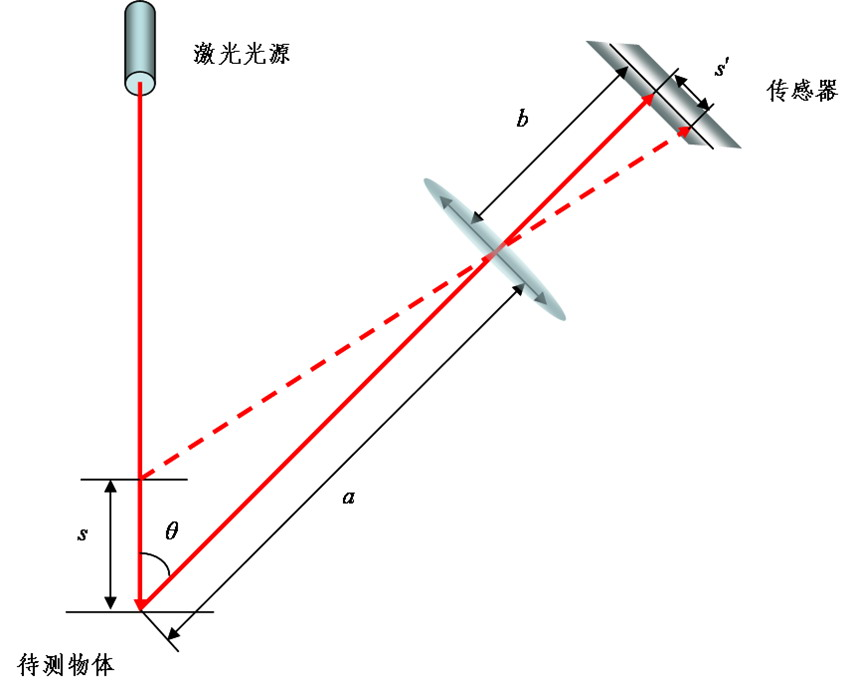
\includegraphics[width=\textwidth]{image/lasertriangulation}
        \caption{\small 激光三角法原理示意图}
        \end{figure}
  \column{3.5cm}
    \begin{itemize}
    \item
    位置关系\\
    $s=\frac{a\cdot s'}{b\cdot \sin \theta \pm s' \cdot \cos \theta}$
    \end{itemize}
  \end{columns}
\end{frame}

\begin{frame}
  \frametitle{新的成像方法}
        \begin{figure}
        \center
        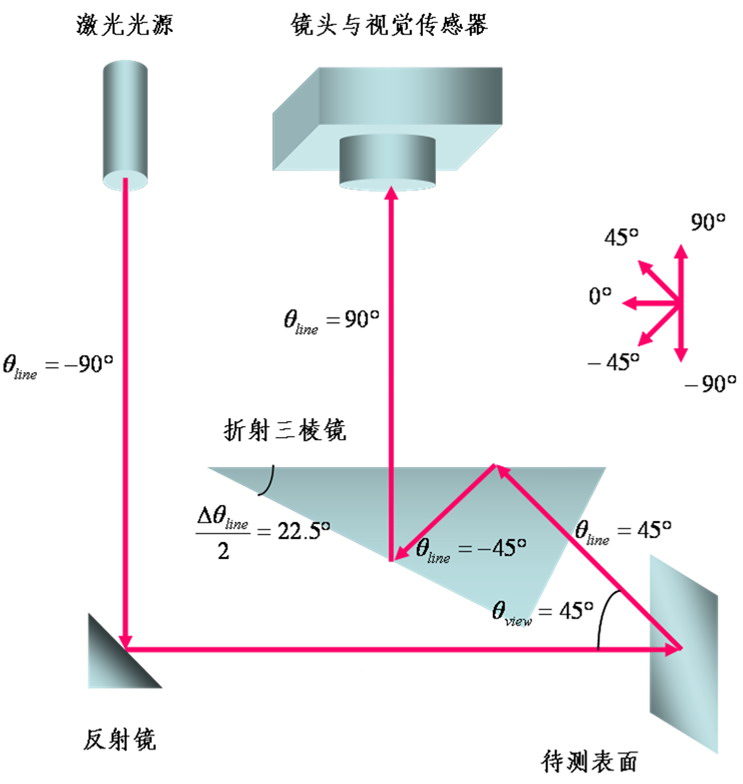
\includegraphics[width=0.5\textwidth]{image/optics}
        \caption{改进方法原理示意图}
        \end{figure}
\end{frame}

\subsection{图像处理与光斑中心定位算法}

\begin{frame}
  \frametitle{图像处理与光斑中心定位流程示意图}
  \begin{overprint}
  \onslide<1>
    \begin{figure}
    \center
    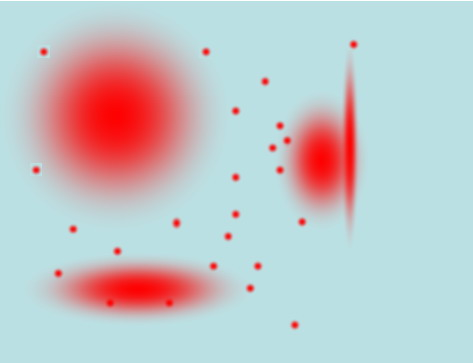
\includegraphics[width=0.6\textwidth]{image/spot1}
    \caption{采集图像}
    \end{figure}
  \onslide<2>
    \begin{figure}
    \center
    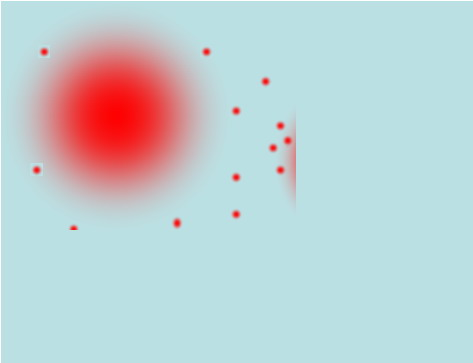
\includegraphics[width=0.6\textwidth]{image/spot2}
    \caption{去除无关区域}
    \end{figure}
  \onslide<3>
    \begin{figure}
    \center
    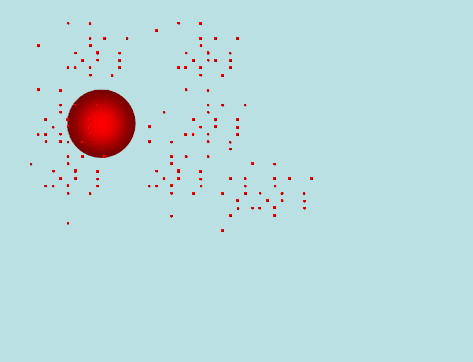
\includegraphics[width=0.6\textwidth]{image/spot3}
    \caption{二值化}
    \end{figure}
  \onslide<4>
    \begin{figure}
    \center
    
\includegraphics[width=0.6\textwidth]{image/spot4}
    \caption{形态学图像处理}
    \end{figure}
  \onslide<5>
    \begin{figure}
    \center
    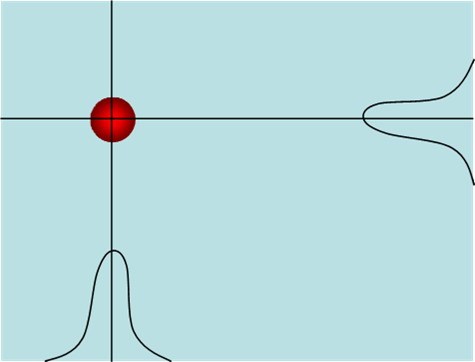
\includegraphics[width=0.6\textwidth]{image/spot5}
    \caption{光斑中心定位}
    \end{figure}
  \end{overprint}
\end{frame}

\section{圆筒检测系统}

\subsection{系统设计与制作}

\begin{frame}
  \frametitle{系统设计图}
    \begin{figure}
    \center
    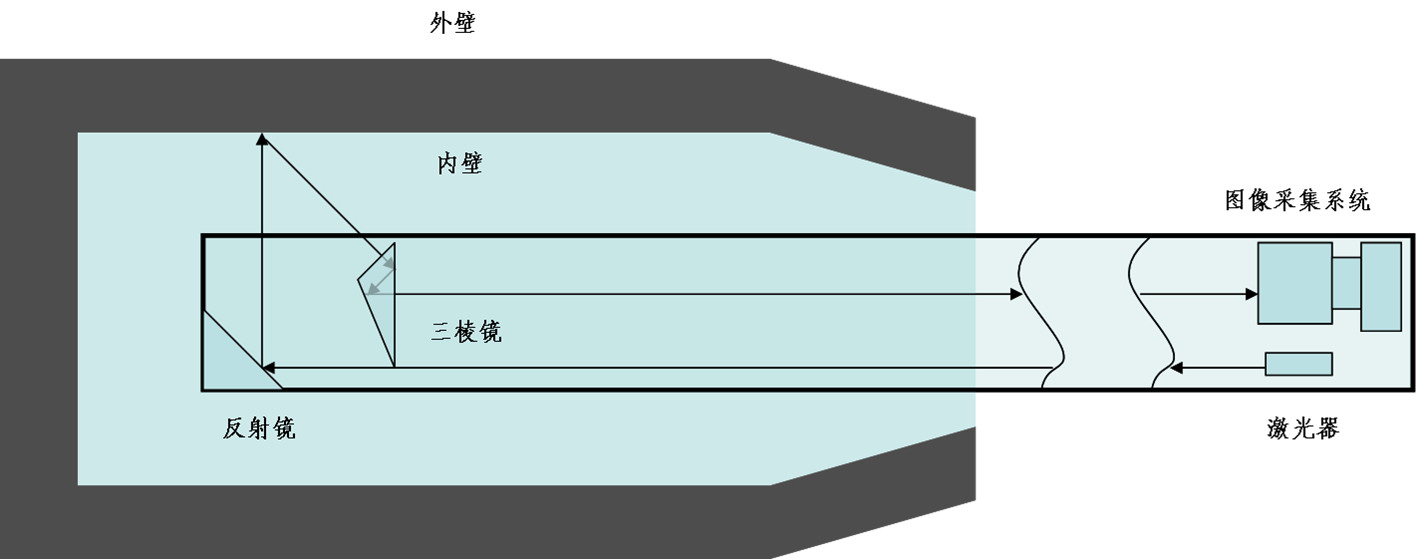
\includegraphics[width=\textwidth]{image/systemmodel}
    \caption{\small 系统组成示意图}
    \end{figure}
\end{frame}

\begin{frame}[label=systemconstitute]
  \frametitle{系统组成}
  \begin{itemize}
  \item
  反射镜:自制。
  \item
  三棱镜:工厂提供。
  \item
  光源:采购华科光电DD650-2.5-5红色点状半导体激光器。
  \item
  镜头:采购Fujinon1/2英寸自动光圈(F=1.8)变焦(7-70mm)FD7V70A镜头。
  \item
  相机:使用松下模拟工业相机。
  \item
  采集卡:使用大恒DH-CG300图像采集卡。
  \item
  机械:与机械学院段振云老师协同设计,在校内工厂加工。
  \end{itemize}

  \hyperlink{machinery<1>}{\beamergotobutton{机械设计图}}
\end{frame}

\begin{frame}
  \frametitle{原型系统}
  \begin{overprint}
  \onslide<1>
    \begin{figure}
    \center
    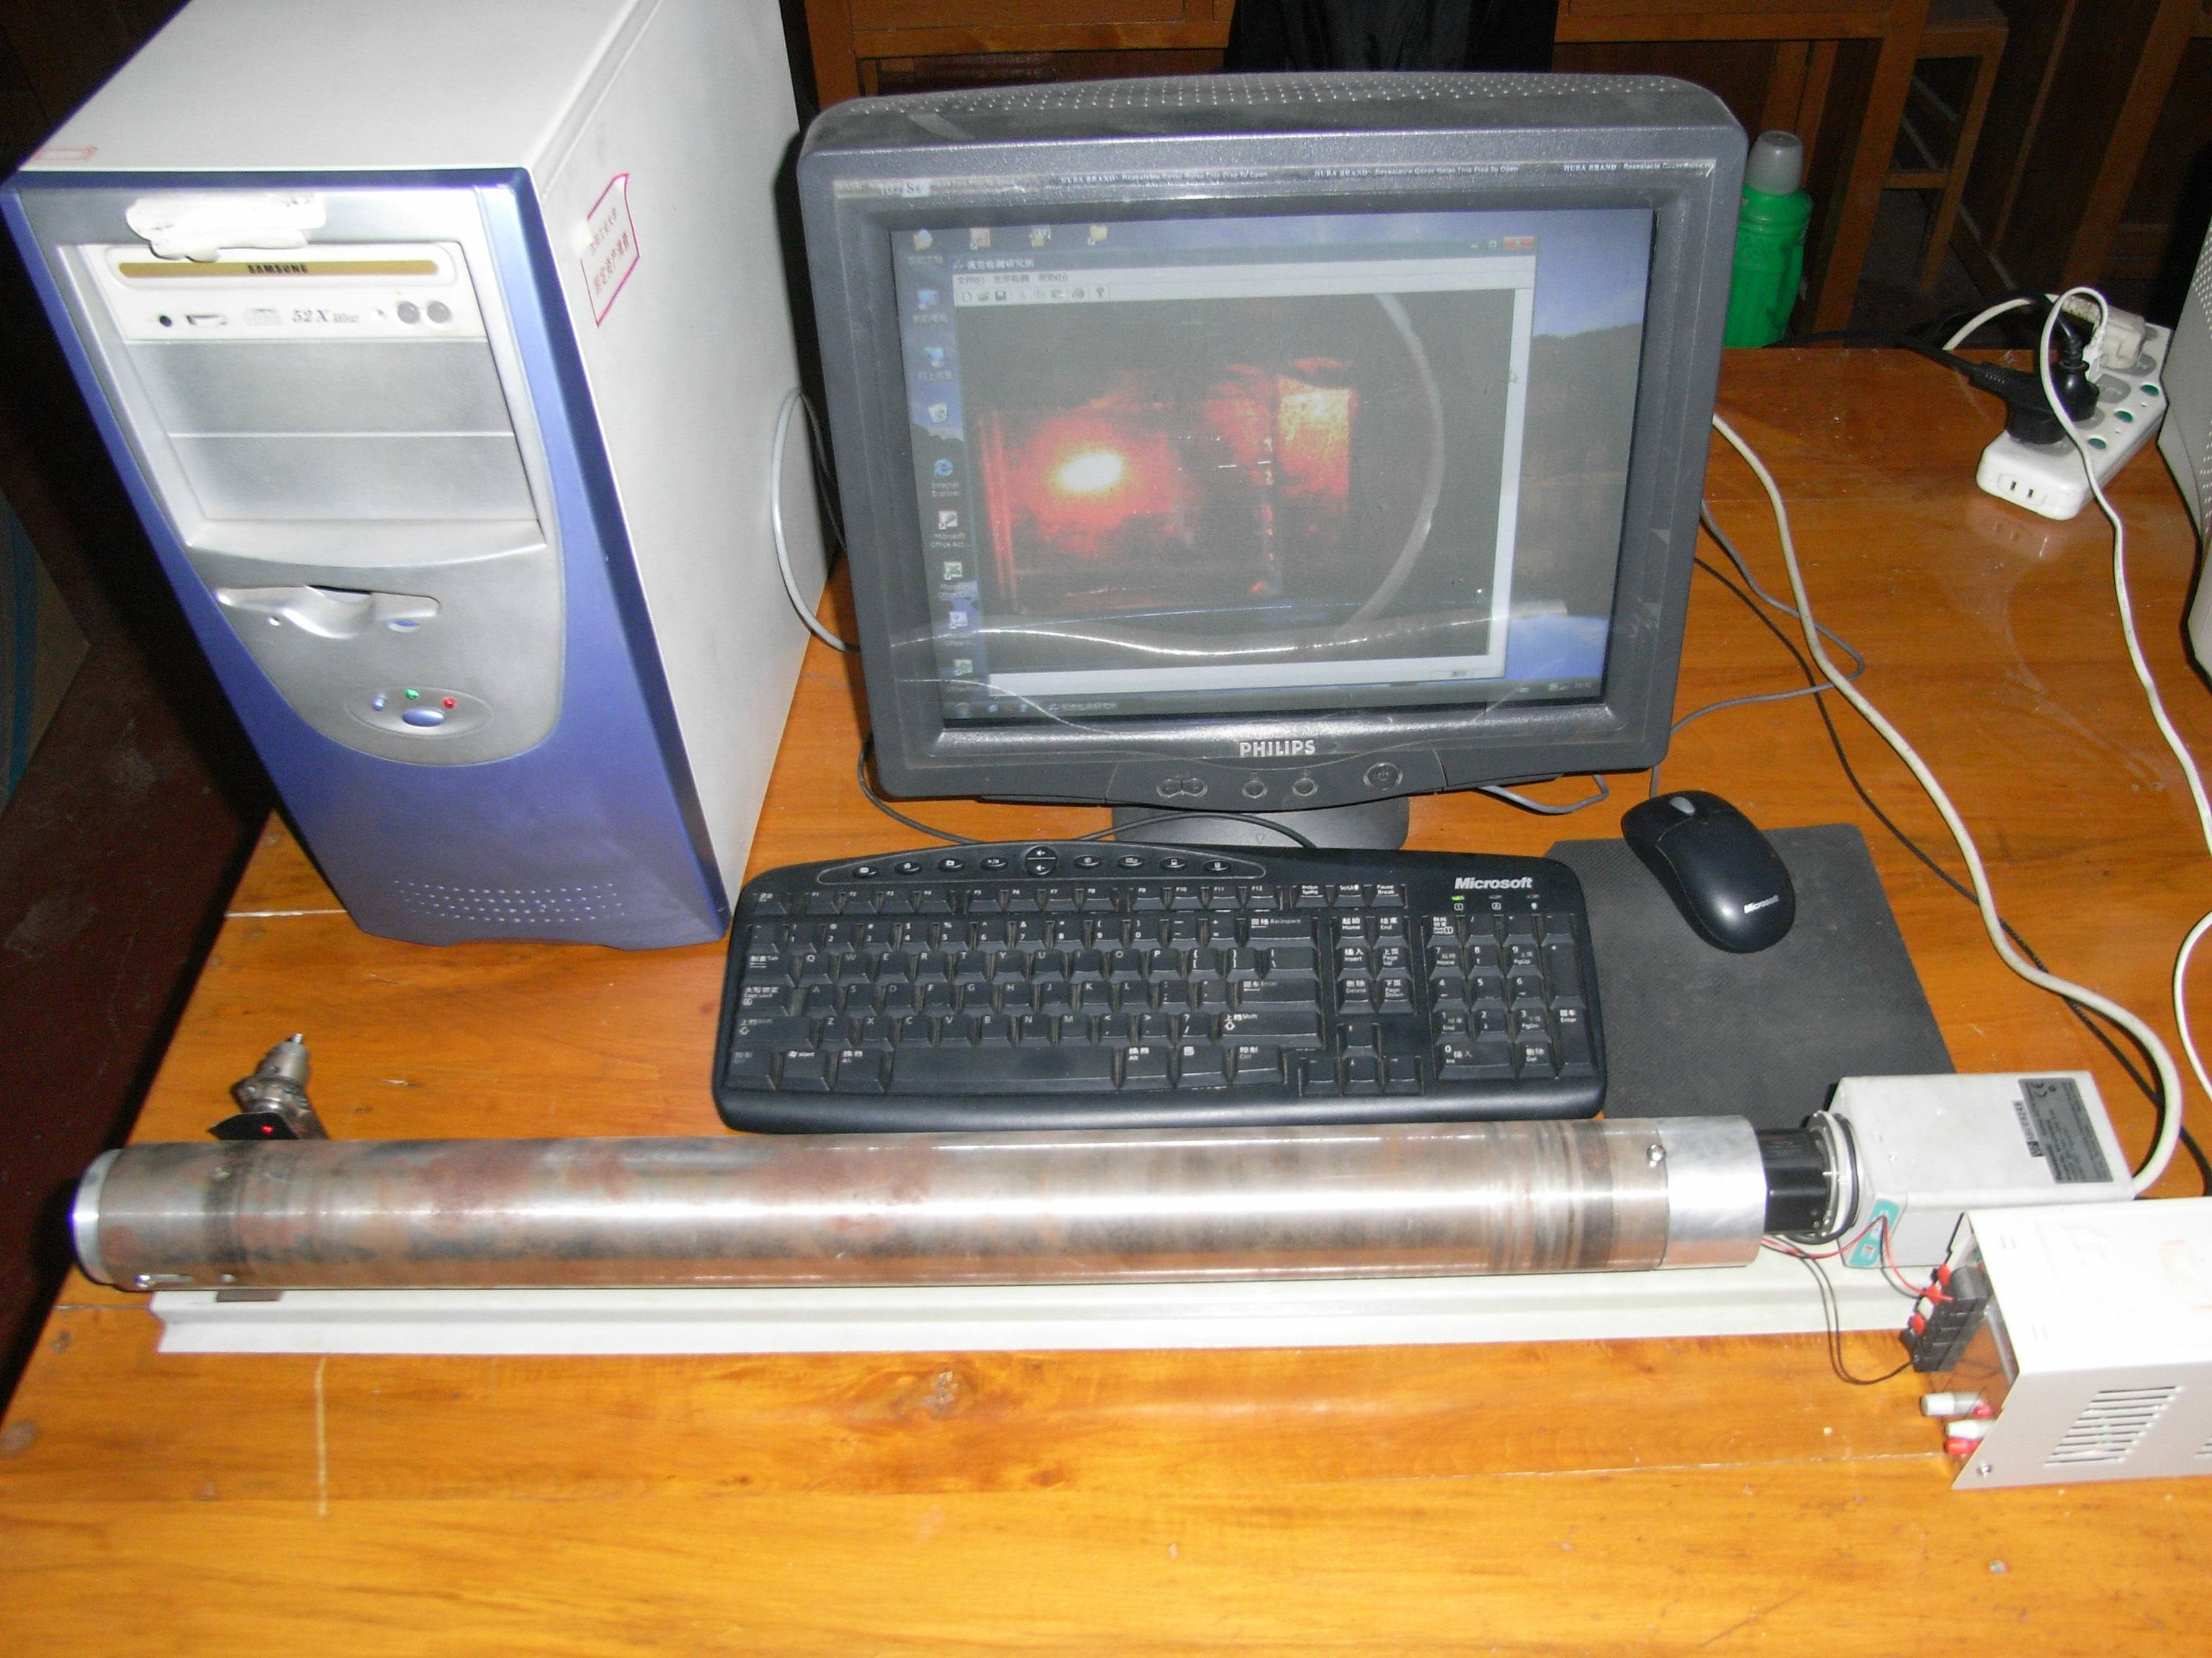
\includegraphics[width=0.7\textwidth]{image/systemworking1}
    \caption{\small 原型系统采集光斑图像}
    \end{figure}
  \onslide<2>
    \begin{figure}
    \center
    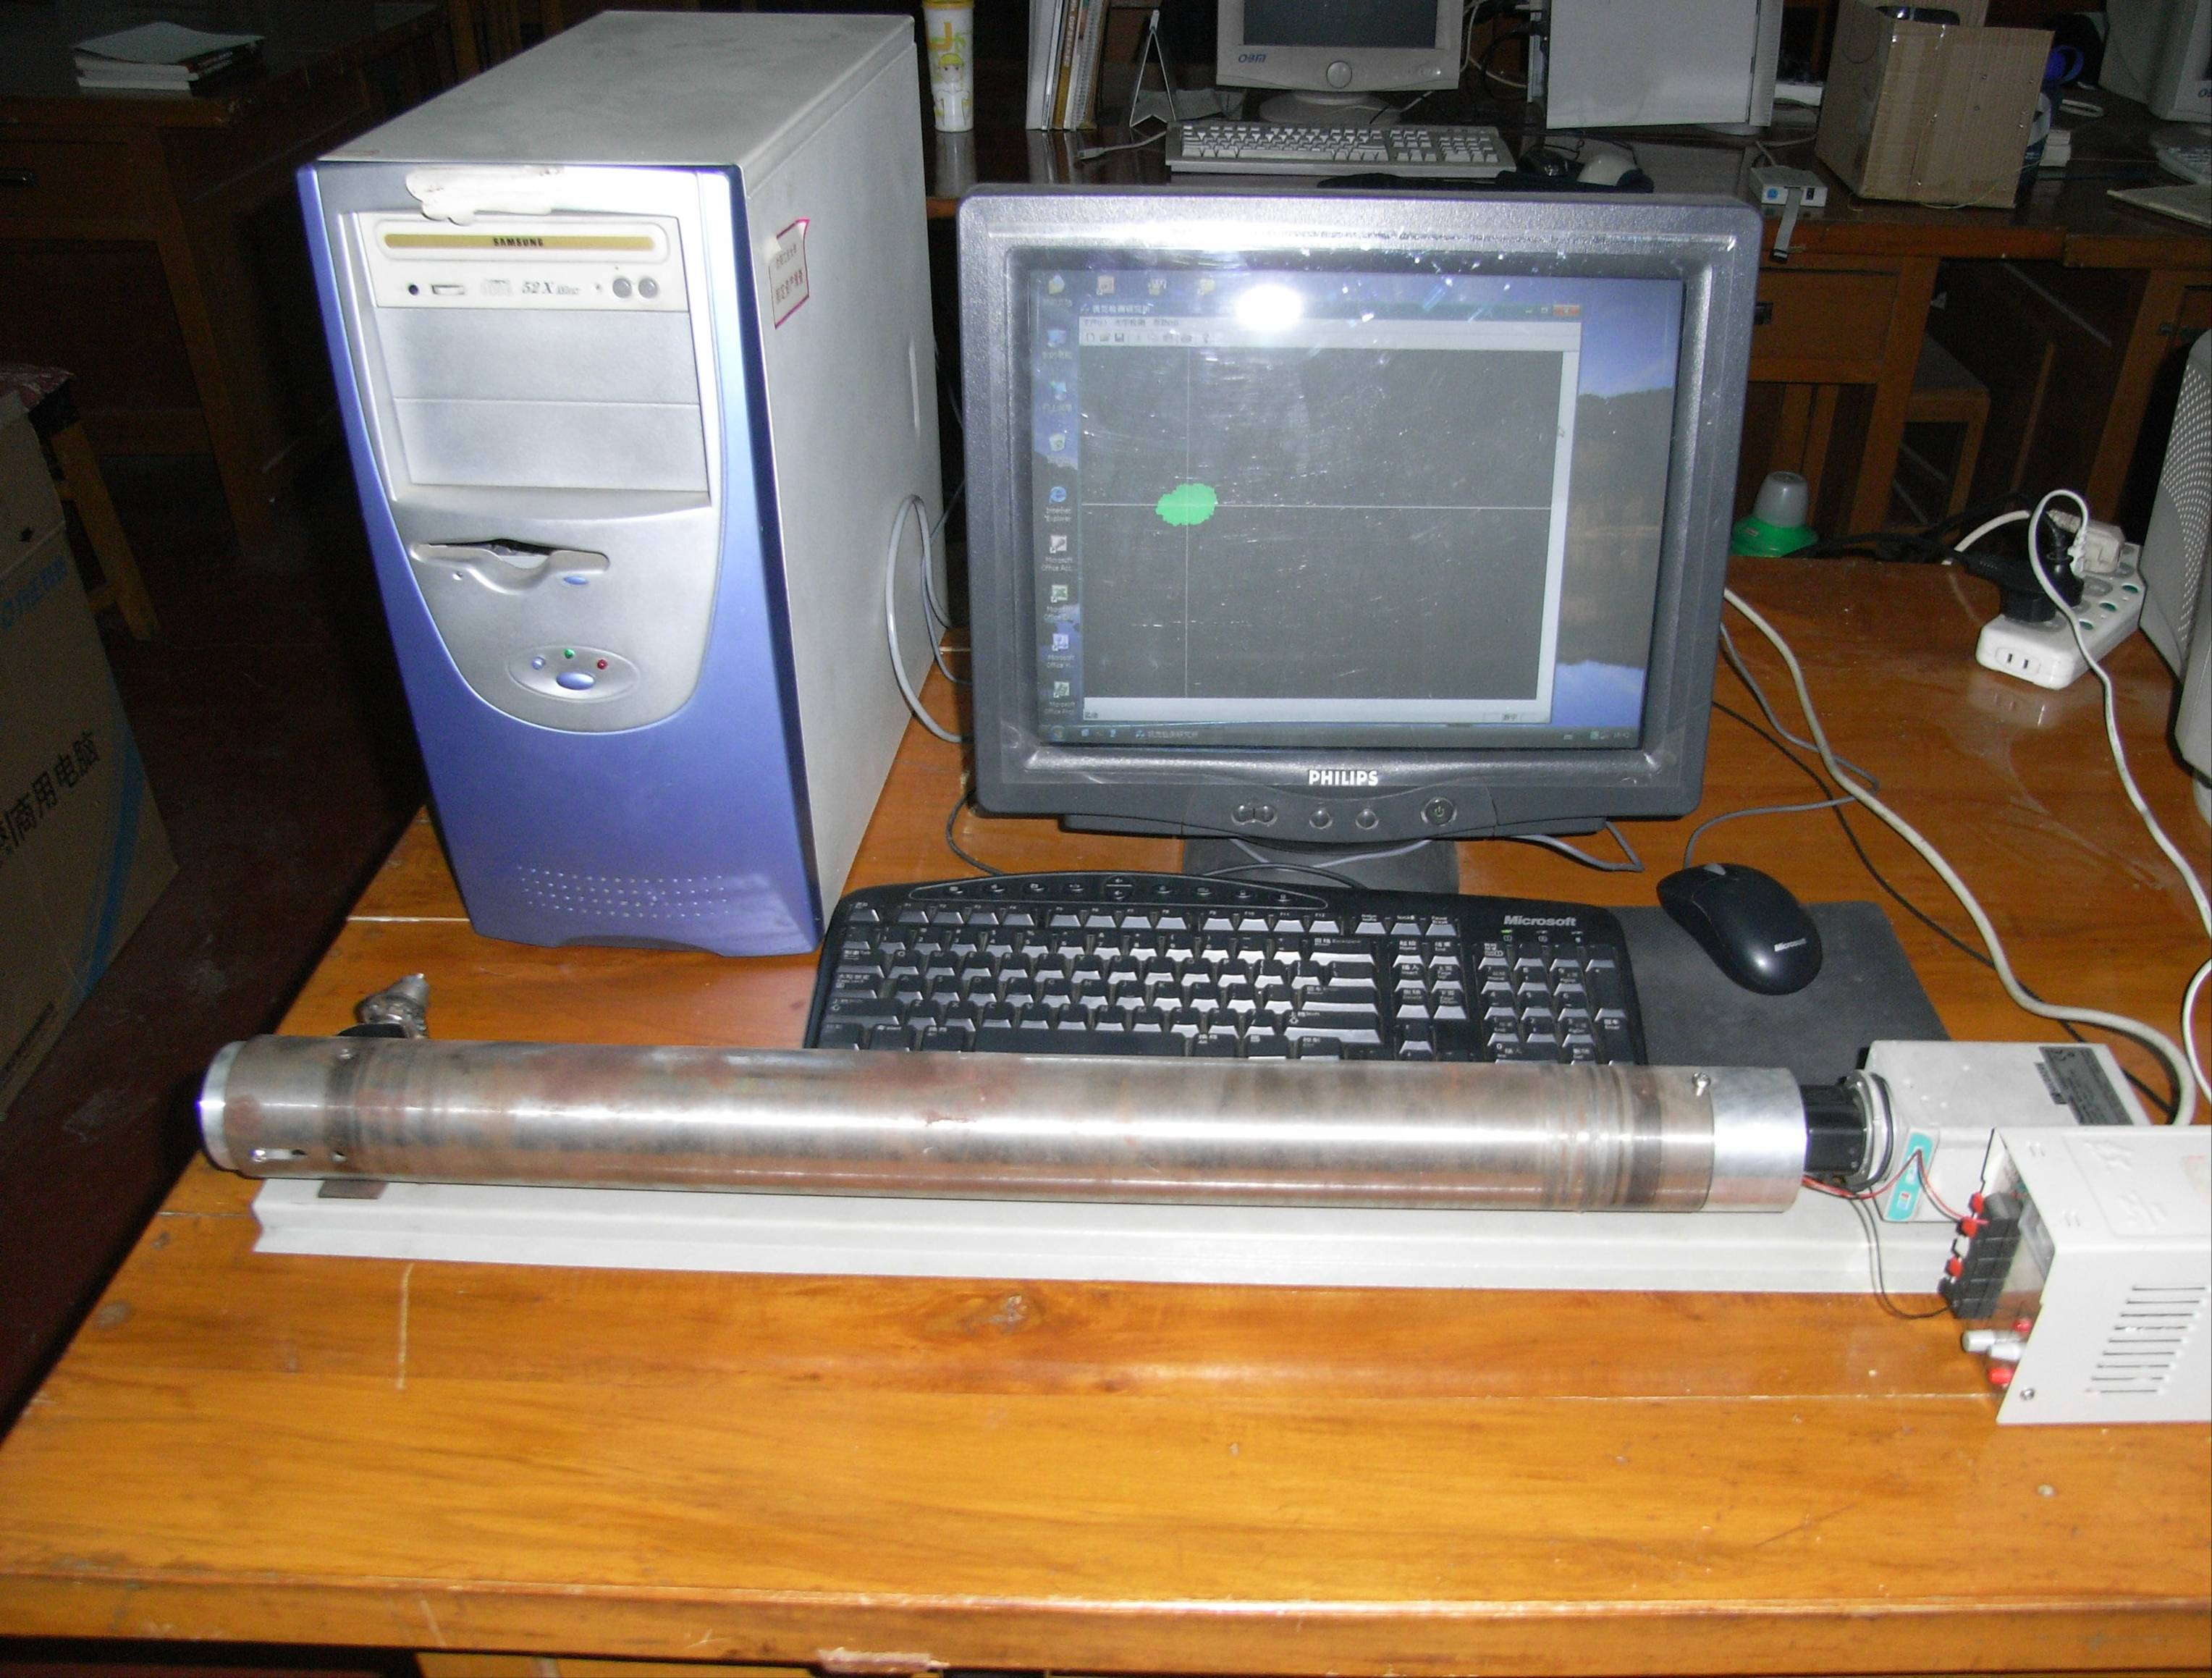
\includegraphics[width=0.7\textwidth]{image/systemworking2}
    \caption{\small 原型系统定位光斑中心}
    \end{figure}
  \onslide<3>
    \begin{figure}
    \center
    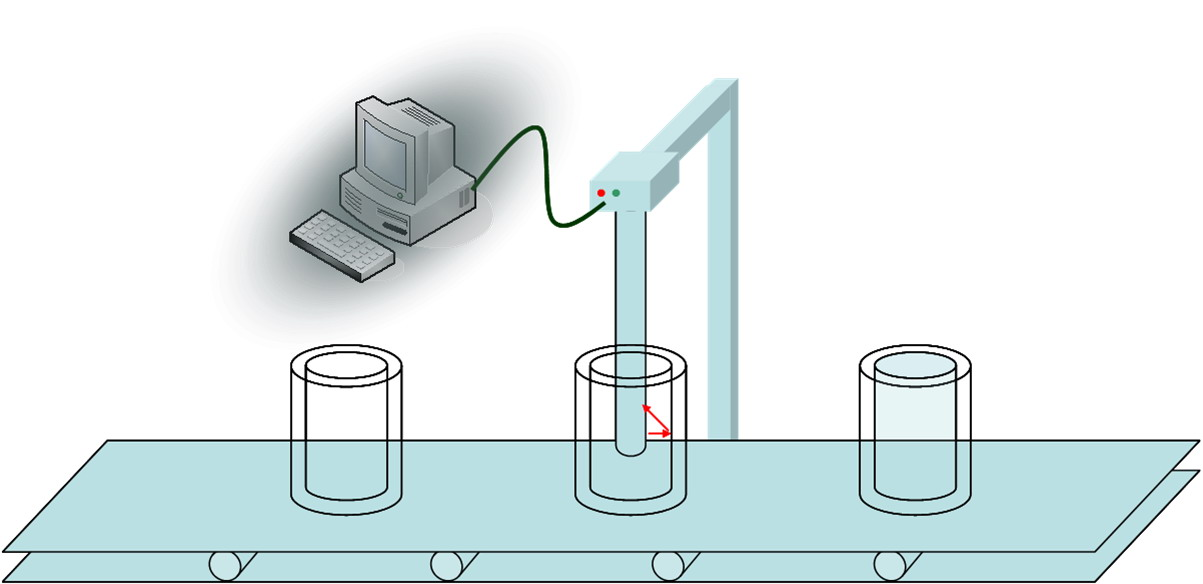
\includegraphics[width=\textwidth]{image/workingmodel}
    \caption{\small 系统工作流程示意图}
    \end{figure}
  \end{overprint}
\end{frame}

\subsection{实验及结论}

\begin{frame}
  \frametitle{实验}
  \begin{overprint}
  \onslide<1>
    \begin{figure}
    \center
    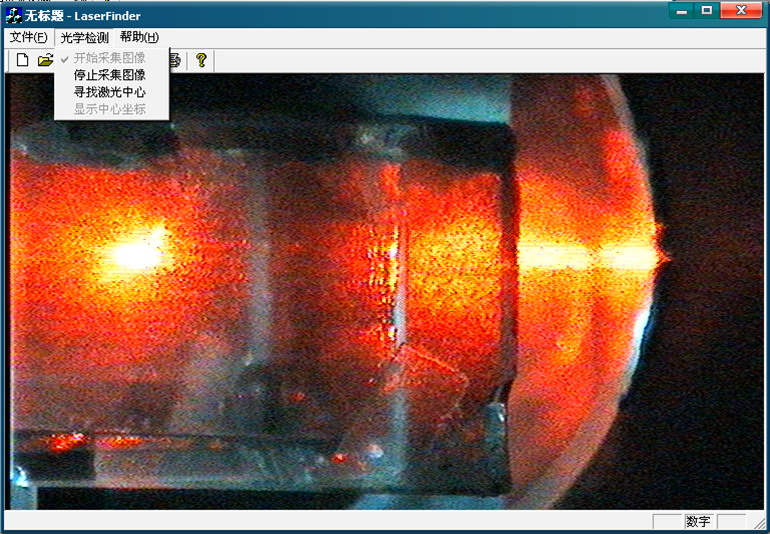
\includegraphics[width=0.7\textwidth]{image/exp1}
    \caption{\small 图像实时采集}
    \end{figure}
  \onslide<2>
    \begin{figure}
    \center
    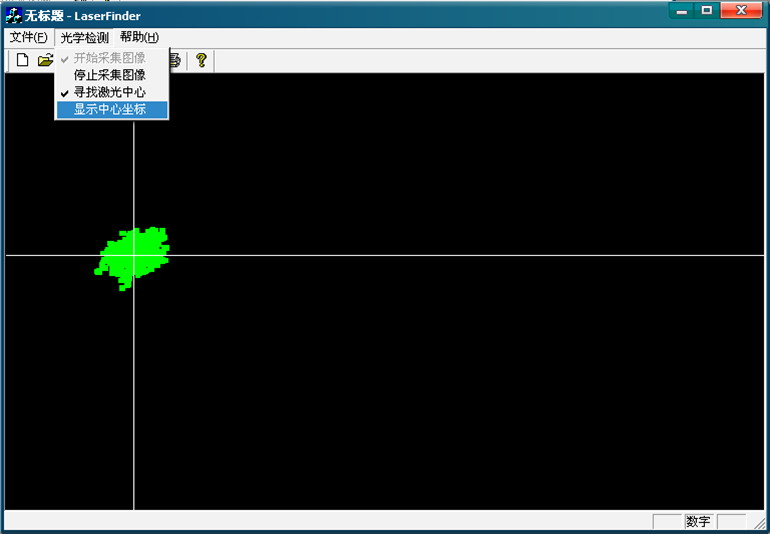
\includegraphics[width=0.7\textwidth]{image/exp2}
    \caption{\small 光斑中心定位}
    \end{figure}
  \onslide<3>
    \begin{figure}
    \center
    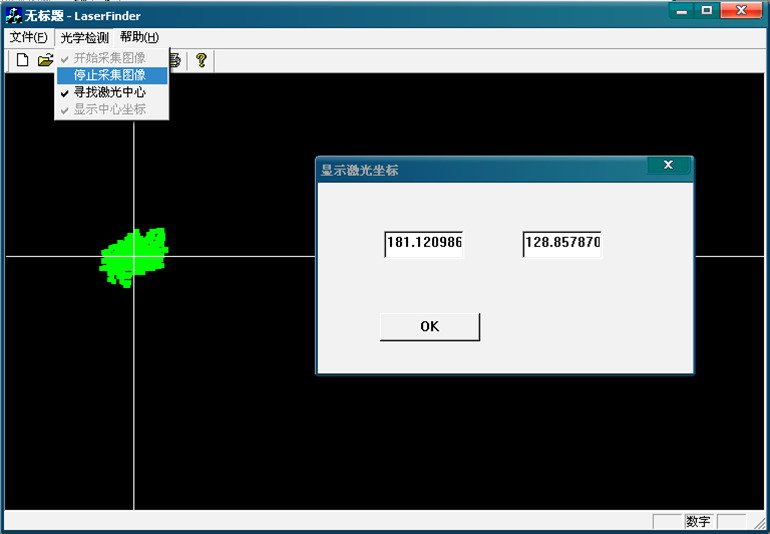
\includegraphics[width=0.7\textwidth]{image/exp3}
    \caption{\small 显示光斑中心坐标}
    \end{figure}
  \end{overprint}
\end{frame}

\begin{frame}[label=conclusion]
  \frametitle{结论}
  \begin{itemize}
  \item
  原型系统实现圆筒实时在线检测\footnote{已获实用新型专利(200620168791.X)并申请发明专利(200610155870.1)}
  \item
  检测分辨率为$0.1mm/pixel$
  \item
  检测范围大于$30mm$
  \item
  检测时间小于$40ms/dot$
  \end{itemize}
  \hyperlink{patent<1>}{\beamergotobutton{在学期间研究成果}}
\end{frame}

\begin{frame}
  \frametitle{有关偏心问题的说明}
    \begin{figure}
    \center
    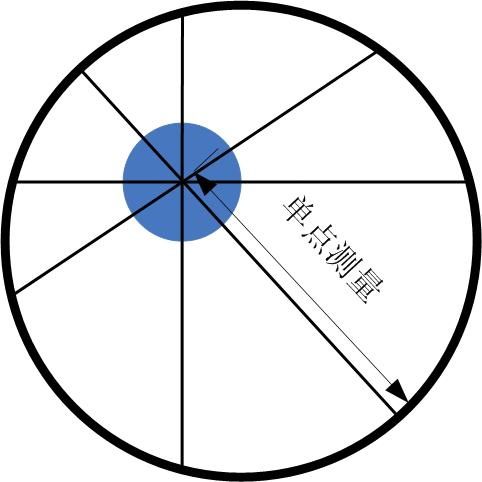
\includegraphics[width=0.5\textwidth]{image/heart}
    \caption{\small 偏心测量原理}
    \end{figure}
\end{frame}

\subsection*{致谢}

\begin{frame}
  \frametitle{\subsecname}
  \begin{columns}
  \column{3.5cm}
  \column{3.5cm}
  \large 谢谢各位老师!
  \column{3.5cm}
  \end{columns}
\end{frame}

\section*{附录}

\subsection*{附录 A}

\begin{frame}[label=patent]
  \frametitle{在学期间研究成果}
  \begin{overprint}
  \onslide<1>
  \begin{block}{专利}
  \begin{enumerate}
  \item
  苑玮琦,曲晓峰,段振云,汤永华,张志佳,桑海峰,圆筒内外壁加工精度在线成像
  检测装置,实用新型专利申请号:200620168791.X,已经提交专利证书费,2月份下
  发专利证书。
  \item
  苑玮琦,曲晓峰,段振云,汤永华,张志佳,桑海峰,圆筒内外壁加工精度在线成像
  检测装置及在线成像检测方法,发明专利申请号:200610155870.1,已经公开。
  \end{enumerate}
  \end{block}
  \onslide<2>
  \begin{block}{论文}
  \begin{enumerate}
  \item
  苑玮琦,曲晓峰,主成分分析重建误差掌纹识别方法,《光学学报》修改后复审。预计
  1月末可以收到录用通知。
  \item
  苑玮琦,曲晓峰,基于视觉的圆筒内外壁均匀度在线检测系统,《仪器仪表学报》在审。
  \item
  苑玮琦,曲晓峰,主成分分析法对几种生物特征提取效果的比较研究,《光学学报》在审。
  \end{enumerate}
  \end{block}
  \onslide<3>
  \begin{block}{获奖}
  \begin{enumerate}
  \item
  曲晓峰,林俊楠,薛丹,王慧利,刘慧,第十届挑战杯飞利浦全国大学生课外学术科技
  作品竞赛三等奖,2007年11月(主办单位:团中央,中国科协,教育部,全国学联,天
  津市政府)。
  \end{enumerate}
  \end{block}
  \end{overprint}
  \hyperlink{conclusion<1>}{\beamergotobutton{back}}
\end{frame}

\subsection*{附录 B}

\begin{frame}[label=machinery]
  \frametitle{机械设计图}
  \begin{overprint}
  \onslide<1>
    \begin{figure}
    \center
    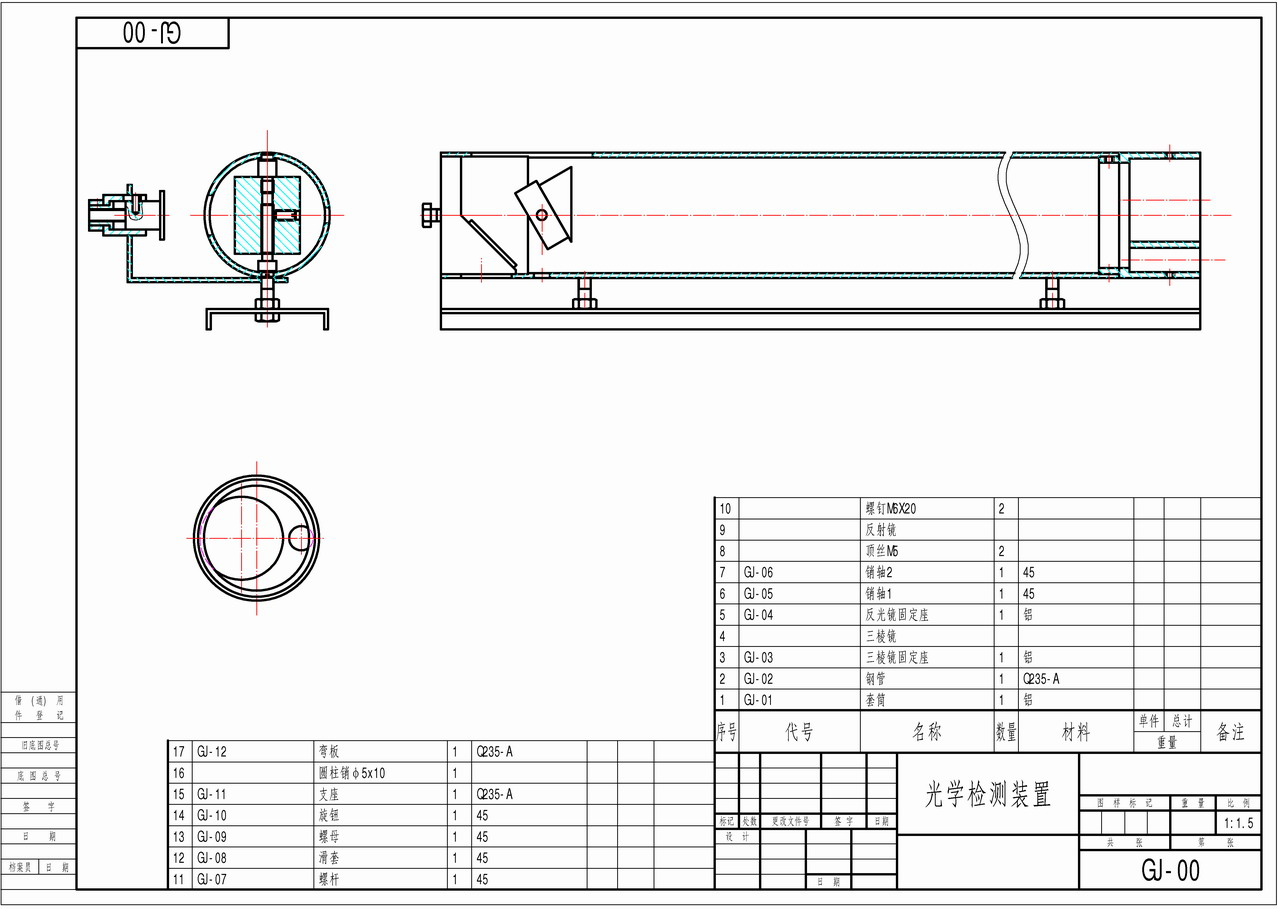
\includegraphics[width=0.7\textwidth]{image/machinery}
    \end{figure}
  \end{overprint}
  \hyperlink{systemconstitute<1>}{\beamergotobutton{back}}
\end{frame}

\subsection*{附录 C}

\begin{frame}[label=story]
  \frametitle{现有科技无法实现}
  \begin{itemize}[<+-| alert@+>]
  \item
  2005年,工厂寻求在线检测方法
  \item
  分别联系国内和国外两家视觉公司
  \item
  经现场考察评估,无法完成该检测任务
  \item
  因此被该厂技术部门评估为\\
  \begin{quote}
  现有科技无法实现
  \end{quote}
  \end{itemize}
  \hyperlink{significance<4>}{\beamergotobutton{back}}
\end{frame}

\end{document}
